\documentclass{template/openetcs_article}
% Use the option "nocc" if the document is not licensed under Creative Commons
%\documentclass[nocc]{template/openetcs_article} 
\usepackage{lipsum,url}
\usepackage{xspace}
\usepackage{graphicx}
\usepackage{fixme}
\usepackage{lscape} 
\usepackage{pgfgantt}
\usepackage{adjustbox}
\usepackage{datetime}



%user specified macros
%\newenvironment{activity}[2][planned]
	{\begin{tabular}{p{0.25\textwidth}@{\hspace{0.05\textwidth}}p{0.7\textwidth}}
			\multicolumn{2}{p{\textwidth}}{\colorbox{black}{\begin{minipage}{1.1cm}\begin{center}\textsc{\footnotesize \textcolor{white}{#1}}\end{center}\end{minipage}}~~\textbf{#2}}\\
	}
	{\end{tabular}}

\newcommand{\entry}[2]{#1:&#2\\}
\newcommand{\website}[1]{Website:&\url{#1}\\}
\newcommand{\desc}[1]{\multicolumn{2}{p{\textwidth}}{#1}\\}

\newcommand{\VV}{Verification \& Validation\xspace}
\newcommand{\vv}{verification \& validation\xspace}

\newcommand{\tbd}{\colorbox{cyan}{\%\%To Be Defined\%\%}}
\newcommand{\tbc}{\colorbox{cyan}{\%\%To Be Confirmed\%\%}}
\newcommand{\todo}[1]{\colorbox{cyan}{\%\%{#1}\%\%}}
\newcommand{\nthng}[1]{}


\graphicspath{{./template/}{.}{./images/}}
\begin{document}
\frontmatter
\project{openETCS}

%Please do not change anything above this line
%============================
% The document metadata is defined below

%assign a report number here
\reportnum{OETCS/WP3/DescriptionOfWork}

%define your workpackage here
\wp{Work Package 3: ``Modelling''}

%set a title here
\title{openETCS Modelling Work Package}

%set a subtitle here
\subtitle{Description of Work}

%set the date of the report here
\date{January 2014}

%define a list of authors and their affiliation here

\author{openETCS WP3 SRS task force}

\affiliation{The Team}
 
%\author{Jan Welte}

%\affiliation{WP3 Safety and Requirements Traceability}

\author{Marielle Petit-Doche}

\affiliation{Methodology}

\author{Uwe Steinke}

\affiliation{Objects)}

\author{Bernd Hekele}

\affiliation{SRS Findings)}

% define the coverart
\coverart[width=350pt]{openETCS_EUPL}

%define the type of report
\reporttype{Description of work}



\begin{abstract}
%define an abstract here

  This work package...



\end{abstract}

%=============================
%Do not change the next three lines
\maketitle
\tableofcontents
\listoffiguresandtables
\newpage
%=============================

% The actual document starts below this line
%=============================


%Start here



%-----------------------------------------------------------------------
\section{Introduction}
%-----------------------------------------------------------------------


\subsection{Motivation}
\label{sec:Motivation}

The openETCS work package WP3 aims to provide the kernel architecture and the design of the openETCS OBU software as mainly specified in UNISIG Subset\_026 version\_3.3.0. 

The appropriate functionality has been divided into a list of functions of different complexity (see \url{https://github.com/openETCS/SRS-Analysis/blob/master/System Analysis/List_Functions.xlsx}).

All these functions are object of the openETCS project and have to be analysed from their requirements and subsequently modelled and implemented. With limited manpower, a reasonable selection and order of these functions is required for the practical work that allows the distribution of the workload, more openETCS participants to join and leads to an executable---limited---kernel function as soon as possible. 

While the first version of this document focuses on the first version of the limited kernel function, it is intended to grow in parallel to the growing openETCS software.


\subsection{Objectives}
\label{sec:Objectives}



The first objective of WP3 software shall be
\begin{itemize}
	\item ``Make the train run as soon as possible, with a very minimum functionality, and in the form of a rapid prototype.''
\end{itemize}
This does not contradict the openETCS goal to conform to EN50128.
\begin{itemize}
	\item After a phase of prototyping, the openETCS software shall be implemented in compliance to EN50128 for SIL4 systems.
\end{itemize}
Additional goals for this document are
\begin{itemize}
	\item Identification of the functions required for a minimum OBU kernel
	\item Architecture overview regarding the minimum OBU kernel
	\item Technical approach: Description of the proceeding and methods to be used
	\item Road map of the minimum OBU kernel functions
	\item Road map thereafter
\end{itemize}

Note: This document will be extended according to the progress of WP3. 





%-----------------------------------------------------------------------
\subsection{Goals of the openETCS Modelling Work}
%-----------------------------------------------------------------------
%\tbc
%by Uwe


\subsubsection{Functional Scope: The Minimum OBU Kernel Function}
\label{sec:FunctionalScopeTheMinimumOBUKernelFunction}

The objective “Make the train run with a very minimum functionality” shall be in terms of on ETCS OBU translated into 
\begin{itemize}
	\item The Train moves on a track equipped with balises and determines its position.
\end{itemize}

That means, for this very first step the train shall not supervise the maximum speed, shall not activate the brakes. Instead, the minimum function set shall be limited to (see \url{https://github.com/openETCS/SRS-Analysis/issues/9} ) 
\begin{itemize}
	\item Receive, filter and manage balise information, received from track (see \url{https://github.com/openETCS/SRS-Analysis/issues/12})
	\item Calculate the actual train position based on balise and odometry information (see \url{https://github.com/openETCS/SRS-Analysis/issues/8})
	\item Calculate the distances between the actual train position to track elements in its front
\end{itemize}

A more detailed architectural breakdown of these functions is available in the form of a SysML model at (see \url{https://github.com/openETCS/modeling/tree/master/model/sysml}. 

In addition, the work on this minimum functionality requires to be supported by
\begin{itemize}
	\item The availability of the ETCS language as specified in Subset UNISIG Subset\_026, chapter 7 and 8
	\item The abiltiy to link intermediate and final results with the requirements of the ETCS specification (subset\_026, ..) 
	\item The usability of a data dictionary (see \url{https://github.com/openETCS/dataDictionary} )
\end{itemize}

These supporting prerequisites are under construction and therefore not completely operable actually. How to deal with these restrictions, will be outlined in chapter ???

\subsubsection{Actual Status}
\label{sec:ActualStatus}

Some first analyis steps for the required minimum functionality have been gone as results from the SRS-Analysis task force. These results are available on \url{https://github.com/openETCS/SRS-Analysis}


\subsubsection{Practical Approach}
\label{sec:PracticalApproach}

The architecture and design of the minimum OBU kernel shall be developed in consideration of the actual status, restricted prerequisites and limited resources as follows. 


\subsection{Organisation of the Work package}

BH: Tasks, Repositories


%-----------------------------------------------------------------------
\section{Methodology}
%-----------------------------------------------------------------------
%\tbc


This section gives some information on how to proceed to achieve the  objectives described in section \ref{sec:Objectives}.
As decided previously in the project, the means chosen to design the WP3 software, compliant to SIL4 requirements of EN50128 are SysML on Papyrus and SCADE for the modelling part, C language for the executive software. The first versions of the OpenETCS toolchain already involve Papyrus.

Other tools can be involved to support the task of the workpackage (indeed to manage requirements, data, traceability,...) but will be defined latter depending of the needs and the propositions.

For further information on means selection and detailed description of the process, consider the deliverables [D7.1]\footnote{\url{https://github.com/openETCS/toolchain/blob/master/T7.1/D7.1/D7.1.pdf}}, [D7.2]\footnote{\url{https://github.com/openETCS/toolchain/blob/master/T7.2/D7.2/D7_2.pdf}} and [D2.4]\footnote{\url{https://github.com/openETCS/requirements/blob/master/D2.4/D2_4.pdf}}.

\subsection{Main step of the analysis}

The figure \ref{fig:Steps} gives the main steps of the design approach and main used and produced artefacts. All is detailed in D2.4.

\begin{figure}[ht]
  \centering
  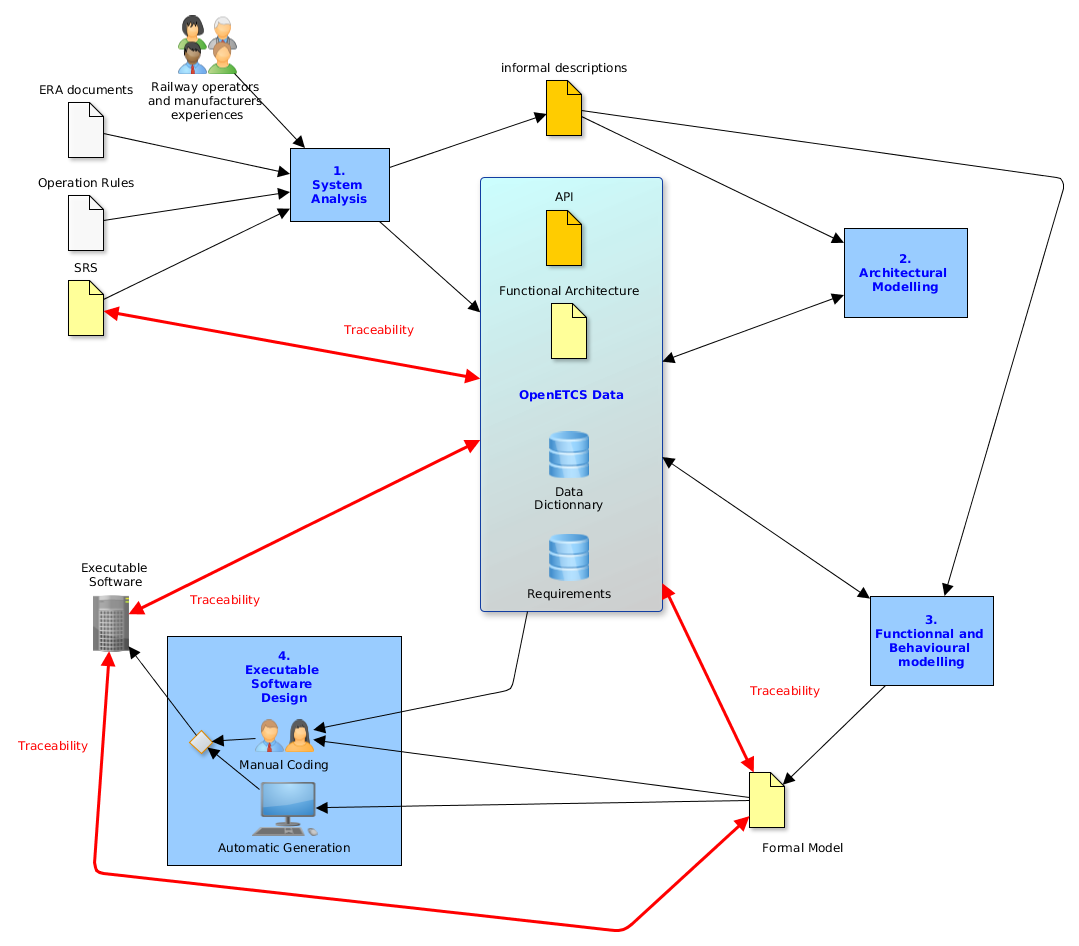
\includegraphics[width=\textwidth]{sections/Step.png}
  \caption{Main steps of the design approach}
  \label{fig:Steps}
\end{figure}


Four main steps are defined:
\begin{description}
\item [System Analysis] to identify the main functions and their interactions and to clarify the requirements allocated to them.
\item [Architectural Modelling] to specify the functional architecture of the system to design and internal and external interfaces. In parallel  the main data exchanged between the functions shall be identified.
\item [Functional and Behavioural Modelling] to provide a formal model of each function.
\item [Executable Software Design] to provide executable part of software.
\end{description}

These steps are sharing common artifacts which going to be updated and completed during all the design phase. Some recommendations and guidelines are defined in D2.4 for naming of elements or specifing a model.

As the artifacts are shared, an iterative process can be easily applied at each level.

\subsection{Shared artifacts}

\subsubsection{Functional architecture and API}

API\footnote{\url{https://github.com/openETCS/requirements/blob/master/D2.7-Technical_Appendix/OETCS_API\ Requirements_v1.0Draft_130301.pdf}} is a document provided as input which can be updated according to the needs.

Functional architecture is specified as a SysML  model, which can be automatically translated in a Scade model. An initial SysML model to cover the initial functional scope \ref{sec:FunctionalScopeTheMinimumOBUKernelFunction} is available on github: \url{https://github.com/openETCS/modeling/tree/master/model/sysml}

See D2.4 for how to use SysML to define the Functional Architecture.

\subsubsection{Set of Requirements}

The initial  set of requirements is the contains of Subset\_026 v3.3.0. These requirements are available as ReqIF format on github: \url{https://github.com/openETCS/modeling/tree/master/model/subset26}
.

This set is going to be increased during the design with updated requirements and added requirements.

Data model of D2.4 gives the information to manage on the requirements.

For the moment, ProR is involved in the openETCS toolchain to define new requirements and links between them.
It is still to clarify how to manage traceability.



\subsubsection{Data Dictionary}

The Data Dictionary is the set of all the types, constants and variables defined to  describe the system.
Data model of D2.4 describes how to define a data.

A preliminary task of the system analysis is to identified and specify the data structure which allow to describe the system.

Then the data structure and data definition shall be implemented in the data dictionary.

For the moment the mean to do this implementation is not clearly identified (UML library ? XML files ?)


\subsubsection{Formal models}

Two  models are provided during this phase:
\begin{itemize}
\item  a semi-formal model in SysML which gives the functional architecture of the system, including interaction between each function  and definition of the data.
\item a formal model in SCADE which follows and completes the same architecture and gives a behavioural description of each function. Then C code can be automatically  generated from this model.
\end{itemize}

\subsection{Function specification and design}


For the specification and the design of a functional block, a set of subtasks can be defined:

\begin{enumerate}
\item Identify the function and the input document to describe it (requirements of subset 26 or other subsets, API,, functional architecture,...)
\item Specify its environment and its external interfaces with an ibd diagram in SysML
\item Define and specify  its internal decomposition in subfunctions and its internal  interfaces with ibd and bdd diagrams in SysML
\item Link and complete to the data dictionary
\item Allocate and manage the requirements
\item Clarify and specify the behavior of each elementary function in SCADE
\item Complete Data dictionary if necessary
\item Complete requirement sets and manage traceability
\item Provide for review
\end{enumerate}



%-----------------------------------------------------------------------
\section{How to handle Findings in the SRS}
%-----------------------------------------------------------------------

%-----------------------------------------------------------------------
\section{How to Handle Findings in the SRS}
%-----------------------------------------------------------------------
%\tbc
by Bernd


\nocite{*}
%===================================================
%Do NOT change anything below this line

\end{document}
